\documentclass[../master]{subfiles}

%\graphicspath{{../eps/}}

\begin{document}

\chapter{中性子コリメータ}
\label{chap::collimator}
\section{ビームサイズを制限する必要性}
中性子ビームは可能な限り細いのもが望ましい.
例えば,半径\SI{50}{\milli\metre}の幅を持っている中性子ビームを用いると,
散乱点が$y$軸方向に\SI{100}{\milli\metre}の幅を持つ.
gridの座標を$y = \SI{0}{\milli\metre}$,plateの座標を$y = \SI{140}{\milli\metre}$とし,
ビームの中心が$y = \SI{70}{\milli\metre}$の位置にあるとすると,
中性子ビームは$y = $\SIrange{20}{120}{\milli\metre}の範囲に入射する.
この時$y = \SI{120}{\milli\metre}$の位置で散乱が起きると,
有感領域はgrid方向に\SI{120}{\milli\metre},plate方向に\SI{20}{\milli\metre}となる.
反対に,$y = \SI{20}{\milli\metre}$の位置で散乱が起きると,
有感領域はgrid方向に\SI{20}{\milli\metre},plate方向に\SI{120}{\milli\metre}となる.
しかし,MAIKo TPC は$y$座標をトラックの周囲に発生した電子が読み出し面に到達する時間差を用いて検出しているため,
$y$座標の絶対値を決定することができない.
すると,図\ref{fig::sensitive_area}のように,
$y = \SI{120}{\milli\metre}$と$y = \SI{20}{\milli\metre}$のどちらで散乱が起きたのかを区別できない.
どちらの場合でも確実に有感領域中で停止したと保証するためには,
散乱点から$y$軸方向に\SI{\pm20}{\milli\metre}を実質の有感領域としなければならない.
\begin{figure}
  \centering
  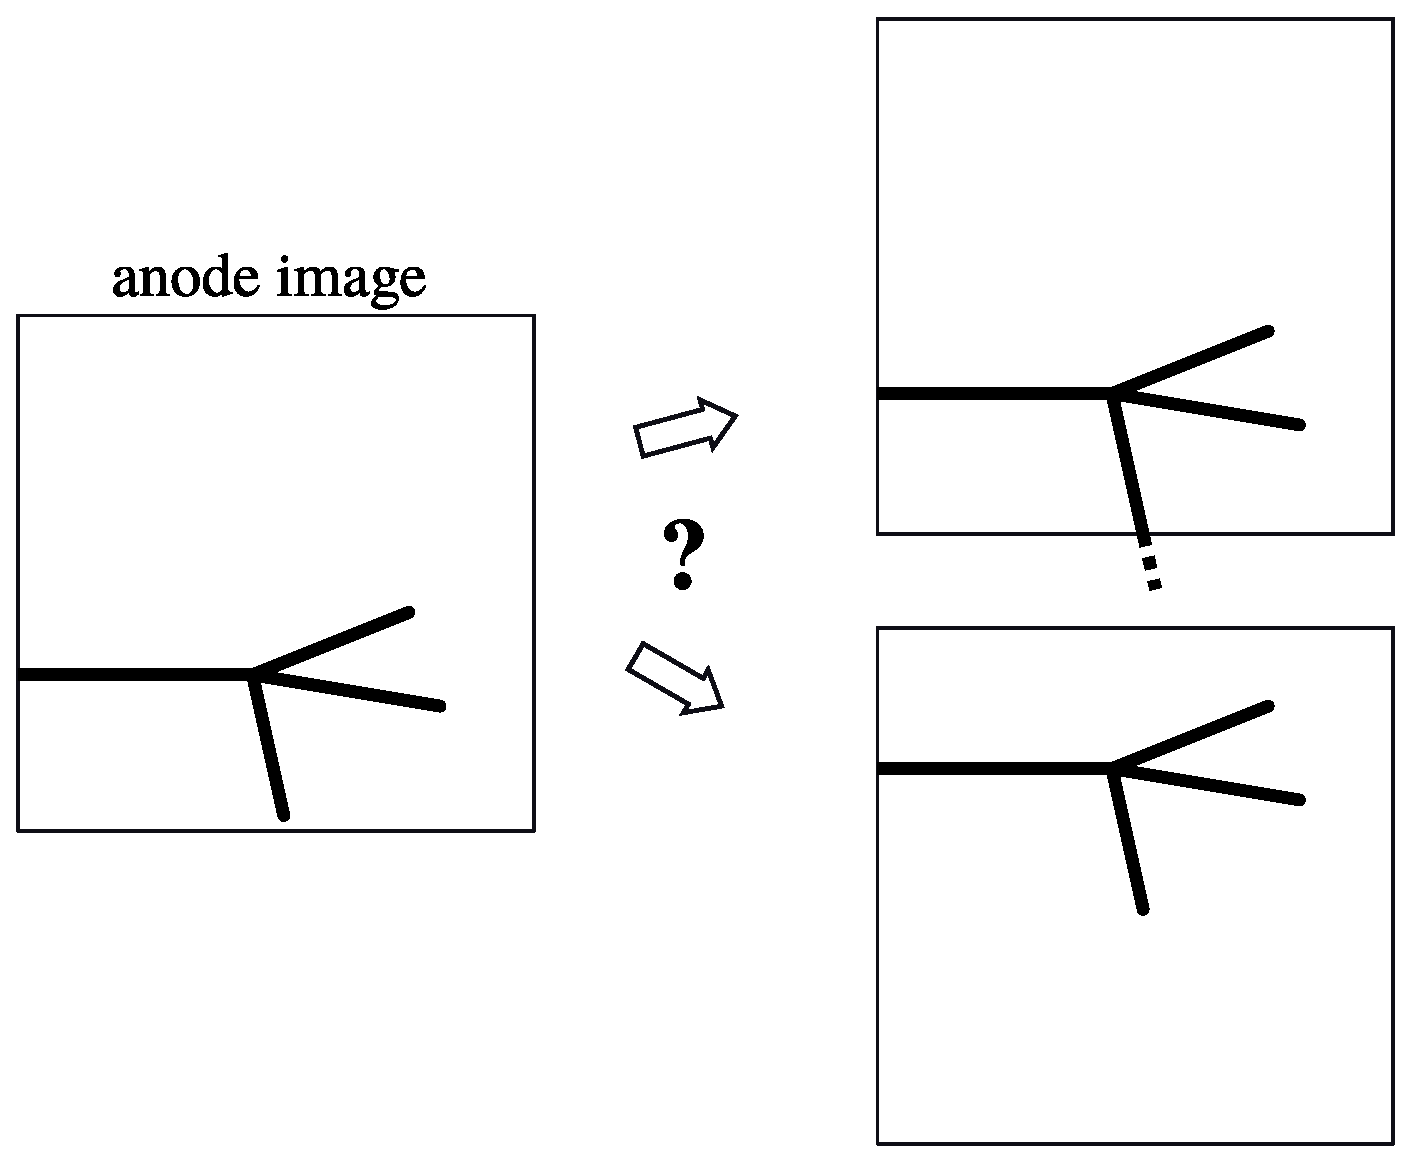
\includegraphics[clip, width=0.6\columnwidth]{sensitive_area.eps}
  \caption[ビームサイズが大きいときの散乱事象.]
          {ビームサイズが大きいときの散乱事象.
            右上のように領域外にトラックが出ているのか,左下のように領域内で停止したのか区別ができない.}
  \label{fig::sensitive_area}
\end{figure}

有感領域が小さいと領域外に出ていく$\alpha$粒子の数が増えてしまい,
検出効率が低下する.
そのため,中性子ビームの$y$軸方向のサイズは可能な限り小さいのもが望ましい.
その反面,ビームを細くすると標的で生成された中性子を制限することになるので,
中性子の入射量が低下する.
%この2つの効果を考慮して収量が大きくなるビームサイズを決定する.

\section{立体角と検出効率によるビームサイズの決定}
重照射室内のトリチウムターゲットから中性子は$4\pi$に等方的に放出していると仮定する.
すると,中性子の収量はコリメータの立体角で決定される.
重照射室の模式図を図\ref{fig::jushosha_room}に示す.
トリチウムターゲットから重照射室の大実験室側の壁までの距離は\SI{1.46e3}{\milli\metre},
壁の厚さは\SI{1e3}{\milli\metre}である.
コリメータの半径を$r$~\si{\milli\metre}とすると,立体角は
$\pi\times r^2/\left(2.46\times10^3\right)^2$となる.
\begin{figure}
  \centering
  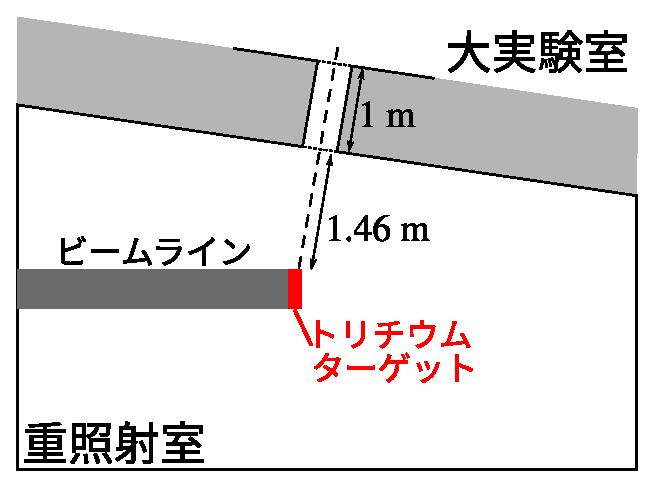
\includegraphics[clip, width=0.7\columnwidth]{jushosha_room.eps}
  \caption{重照射室の模式図.トリチウムターゲットから大実験室まで\SI{2.46}{\metre}である.}
  \label{fig::jushosha_room}
\end{figure}

MAIKo TPC ではトラックの長さと方向からエネルギーと運動量を決定するため,
トラック全体を正しく抽出することが必要となり,MAIKo TPC の有感領域内で停止しない$\alpha$粒子は解析に用いることができない.
ここで,MAIKo TPC の有感領域中で全ての$\alpha$粒子が停止する割合を検出効率とする.
検出効率が大きくなるような実験条件が望ましい.
図\ref{fig::alpha_E_dist}のエネルギー分布,ビームの通る円柱内で一様な散乱点を仮定して,
$\alpha$粒子の検出効率を求めた.
\SIrange{5}{50}{\milli\metre}でのコリメータの立体角の割合と検出効率を
表\ref{tab::solid_angle_percent}に示す.
検出効率は\SI{10}{\milli\metre}以下ではあまり変化がない.
\SI{5}{\milli\metre}と\SI{10}{\milli\metre}を比較すると,
立体角は\SI{10}{\milli\metre}の方が4倍大きい.
大きな検出効率を持ちつつ,中性子の収量が大きい\SI{10}{\milli\metre}のコリメータを用いる.
%コリメータの立体角と検出効率の積が最も大きくなるところが収量が最も大きくなる.
\begin{table}
  \centering
  \caption{コリメータの半径とコリメータの立体角,検出効率.}
  \label{tab::solid_angle_percent}
  \begin{tabular}{ccc}
    \toprule
    コリメータの半径 (\si{\milli\metre}) & 立体角 (\si{\steradian}) & 検出効率 (\si{\percent})\\% & 積\\
    \midrule
     5 & $1.30\times10^{-5}$ & 48.7 \\%& $6.33\times10^{-6}$ \\
    10 & $5.19\times10^{-5}$ & 48.2 \\%& $2.50\times10^{-5}$ \\
    20 & $2.08\times10^{-4}$ & 46.6 \\%& $9.69\times10^{-5}$ \\
    30 & $4.67\times10^{-4}$ & 39.2 \\%& $1.83\times10^{-4}$ \\
    40 & $8.31\times10^{-4}$ & 26.3 \\%& $2.19\times10^{-4}$ \\
    50 & $1.30\times10^{-3}$ & 10.3 \\%& $1.34\times10^{-4}$ \\
    \bottomrule
  \end{tabular}
\end{table}

\section{コリメータの材質}
中性子を遮蔽する材料として,陽子を多く含むポリエチレンや吸収断面積が大きいホウ素が広く用いられている.
ポリエチレンとホウ素入りポリエチレンでの中性子の遮蔽度合いをPHITS (Particle and Heavy Ion Transport code System)
ver.~3.14~\cite{phits}を用いて計算した.
PHITS は原子力機構が中心となって開発を行っている物質中での放射線の挙動をシミュレートするモンテカルロ計算コードである.
PHITS の入力ファイルを付録\ref{chap::phits-input}に示す.
図\ref{collimator_xy_pos}は\SI{14}{\mega\electronvolt}の中性子がコリメータを通過したときの位置分布である.
%ポリエチレンとホウ素入りポリエチレンの両方共,半径\SI{10}{\milli\metre}のみ多くの中性子が通過していることが分かる.
%また,遮蔽されている部分は中心と比較して1桁以上中性子の量が少ないことが分かる.
%2つの中性子の分布に大きな差異は見られない.
図\ref{fig::neutron_energy}はコリメータを通過した後の中性子のエネルギー分布である.
青色のヒストグラムは\SIrange{0}{10}{\milli\metre}の範囲の中性子,
赤色のヒストグラムは\SIrange{10}{55}{\milli\metre}の範囲の中性子のエネルギー分布である.
ポリエチレン,ホウ素入りポリエチレンともにコリメータの穴の部分に対して遮蔽されている部分は
中性子の量が2桁近く少ないことが分かる.
また,通過してきた中性子のエネルギーはほとんど\SI{14}{\mega\electronvolt}であり,
単色エネルギーが汚れていないことが分かる.
\begin{figure}
  \centering
  \begin{subfigure}{\columnwidth}
    \centering
    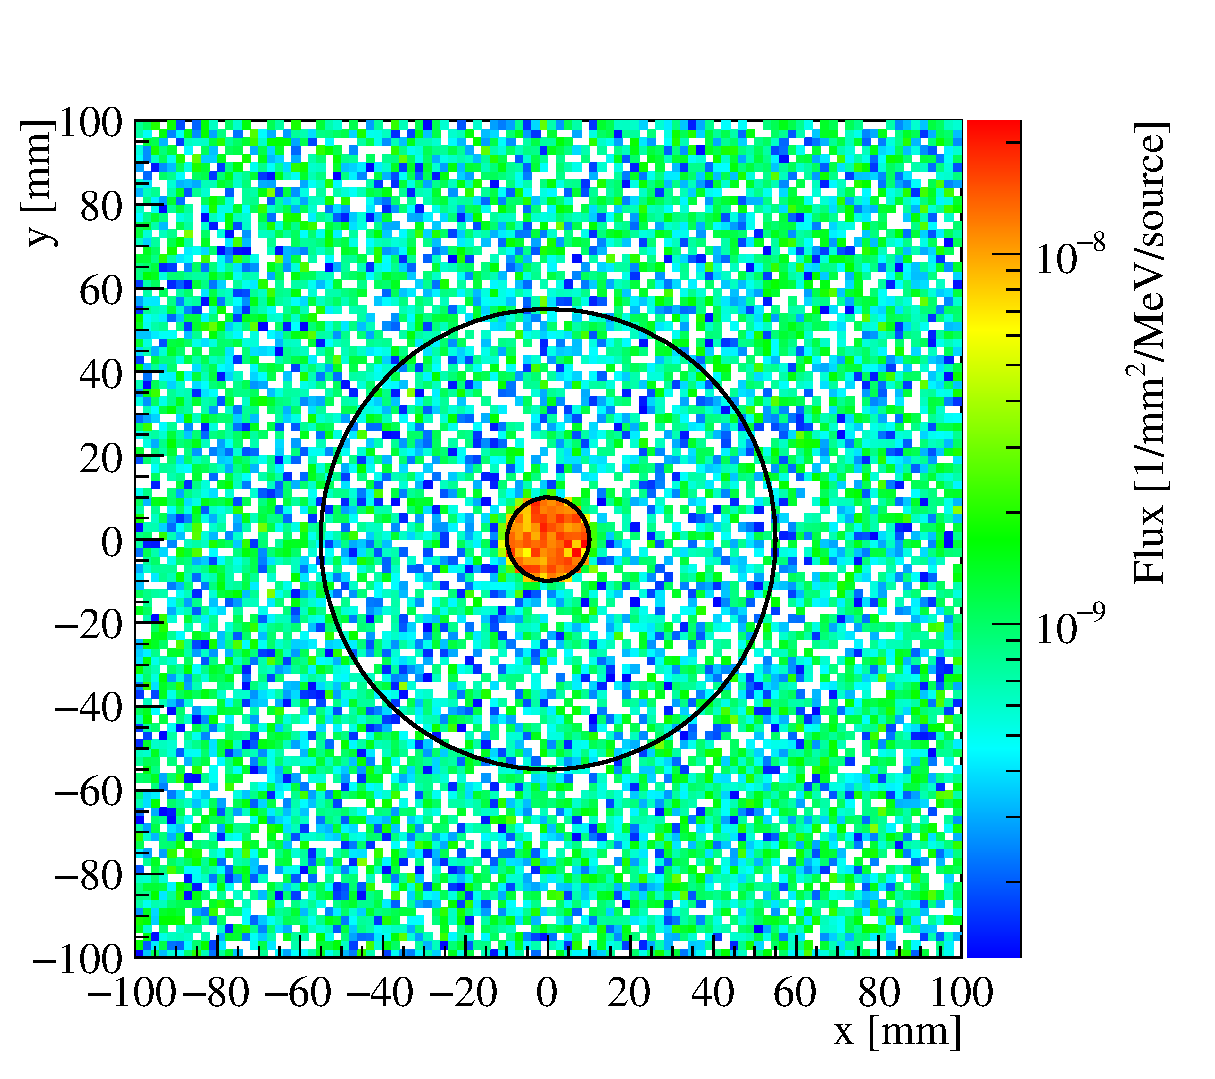
\includegraphics[clip, width=0.7\columnwidth]{cross_xy_f_w_l.eps}
    \caption{ポリエチレンの場合.}
  \end{subfigure}
  \begin{subfigure}{\columnwidth}
    \centering
    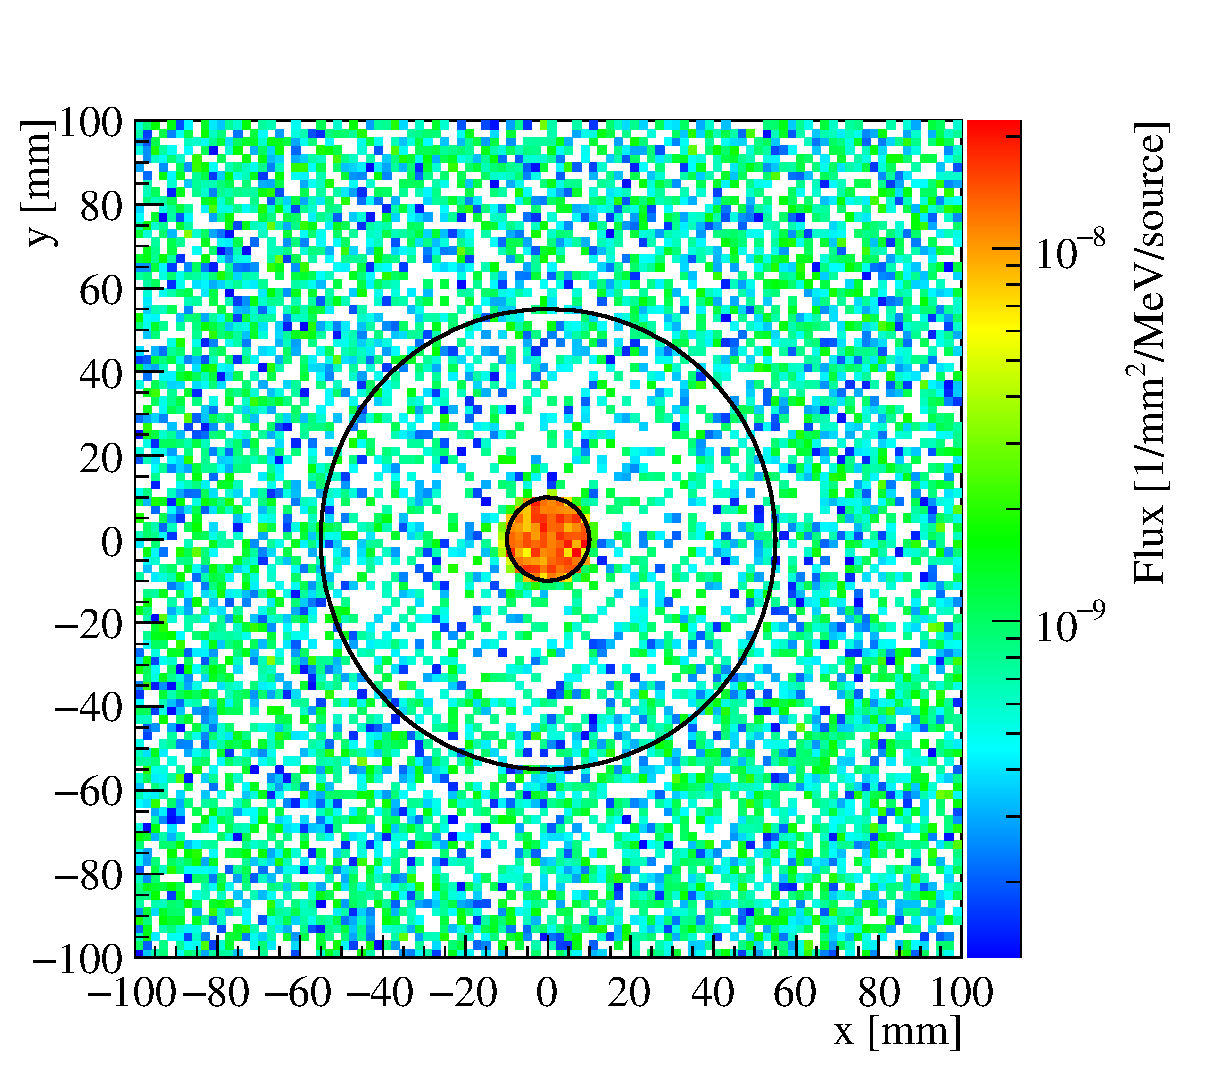
\includegraphics[clip, width=0.7\columnwidth]{cross_xy_f_w_B_w_l.eps}
    \caption{ホウ素入りポリエチレンの場合.}
  \end{subfigure}
  \caption[コリメータ通過後の中性子の位置分布.]
          {コリメータ通過後の中性子の位置分布.2つの円はコリメータの穴と外縁を表す.}
  \label{collimator_xy_pos}
\end{figure}
\begin{figure}
  \begin{subfigure}{\columnwidth}
    \centering
    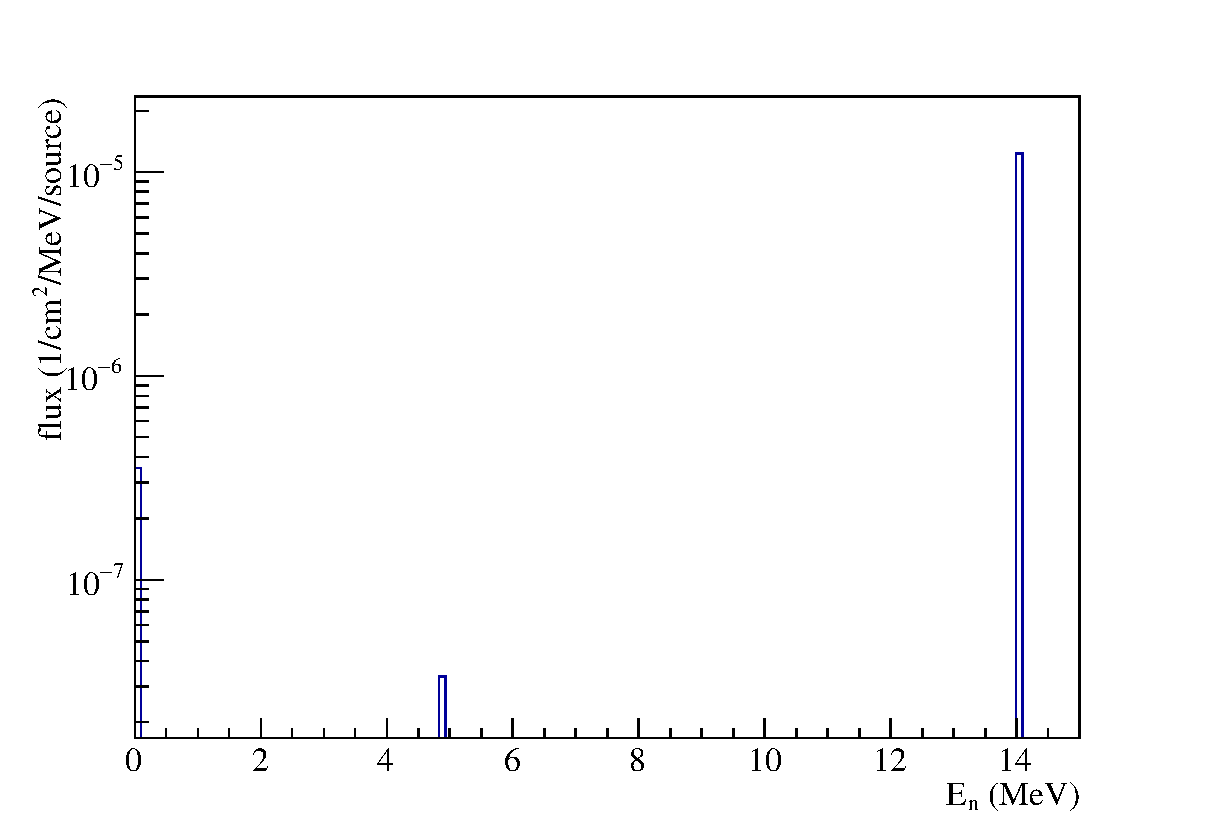
\includegraphics[clip, width=0.8\columnwidth]{cross_eng_f.eps}
    \caption{ポリエチレンコリメータの場合.}
    \label{fig::neutron_energy_dist}
  \end{subfigure}
  \begin{subfigure}{\columnwidth}
    \centering
    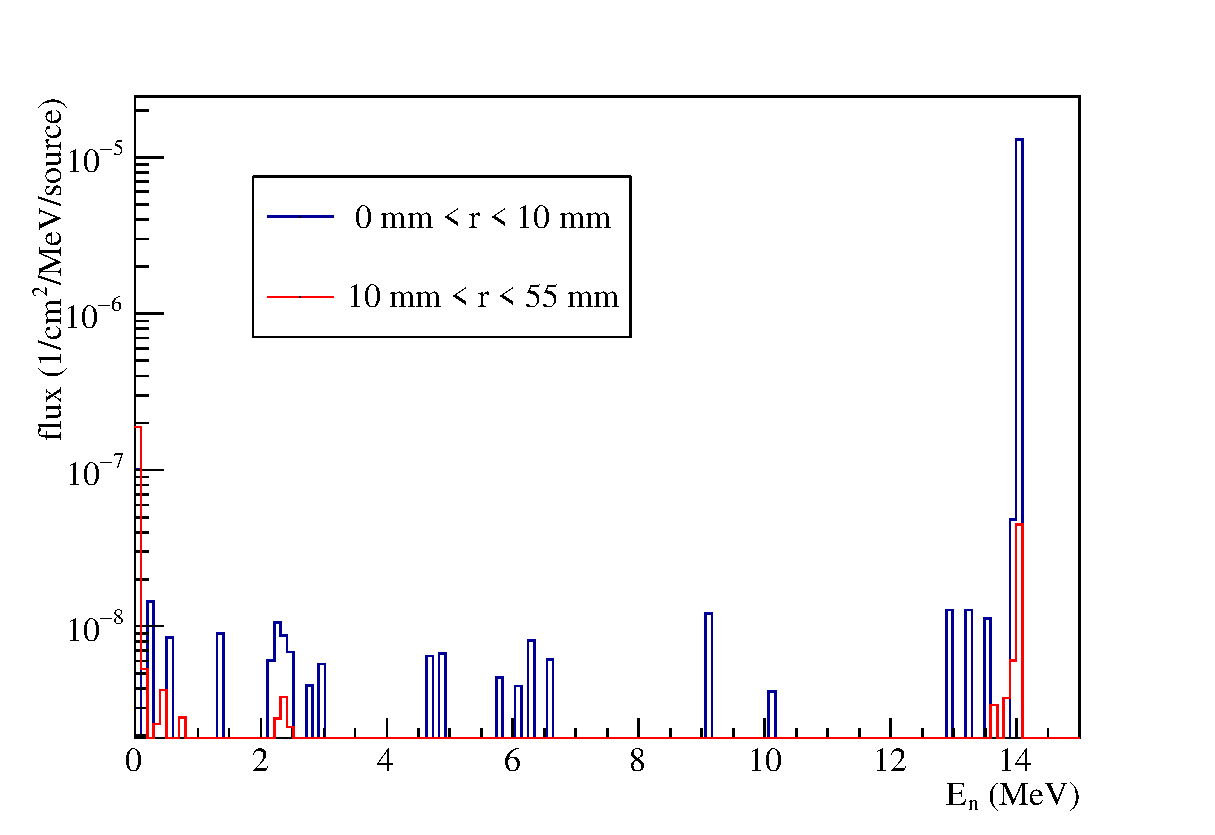
\includegraphics[clip, width=0.8\columnwidth]{cross_eng_f_w_B.eps}
    \caption{ホウ素入りポリエチレンコリメータの場合.}
    \label{fig::neutron_energy_dist_w_B}
  \end{subfigure}
  \caption[中性子のエネルギー分布.]
          {中性子のエネルギー分布.\SIrange{0}{10}{\milli\metre}はコリメータの穴の部分,
          \SIrange{10}{55}{\milli\metre}はコリメータの部分である.}
  \label{fig::neutron_energy}
\end{figure}

ポリエチレンとホウ素入りポリエチレンでは同程度にコリメートできているので,
本実験ではコストの面からポリエチレンを用いたコリメータを作成した.
実際に作成したコリメータを図\ref{pic::collimator}に示す.
このコリメータは半径\SI{53}{\milli\metre},高さ\SI{100}{\milli\metre}の円柱の中心に
半径\SI{10}{\milli\metre}の穴を開けた構造になっている.
壁の厚さが\SI{1000}{\milli\metre}であるため,
このコリメータ10 個を中性子の取り出し穴に挿入する.
\begin{figure}
  \centering
  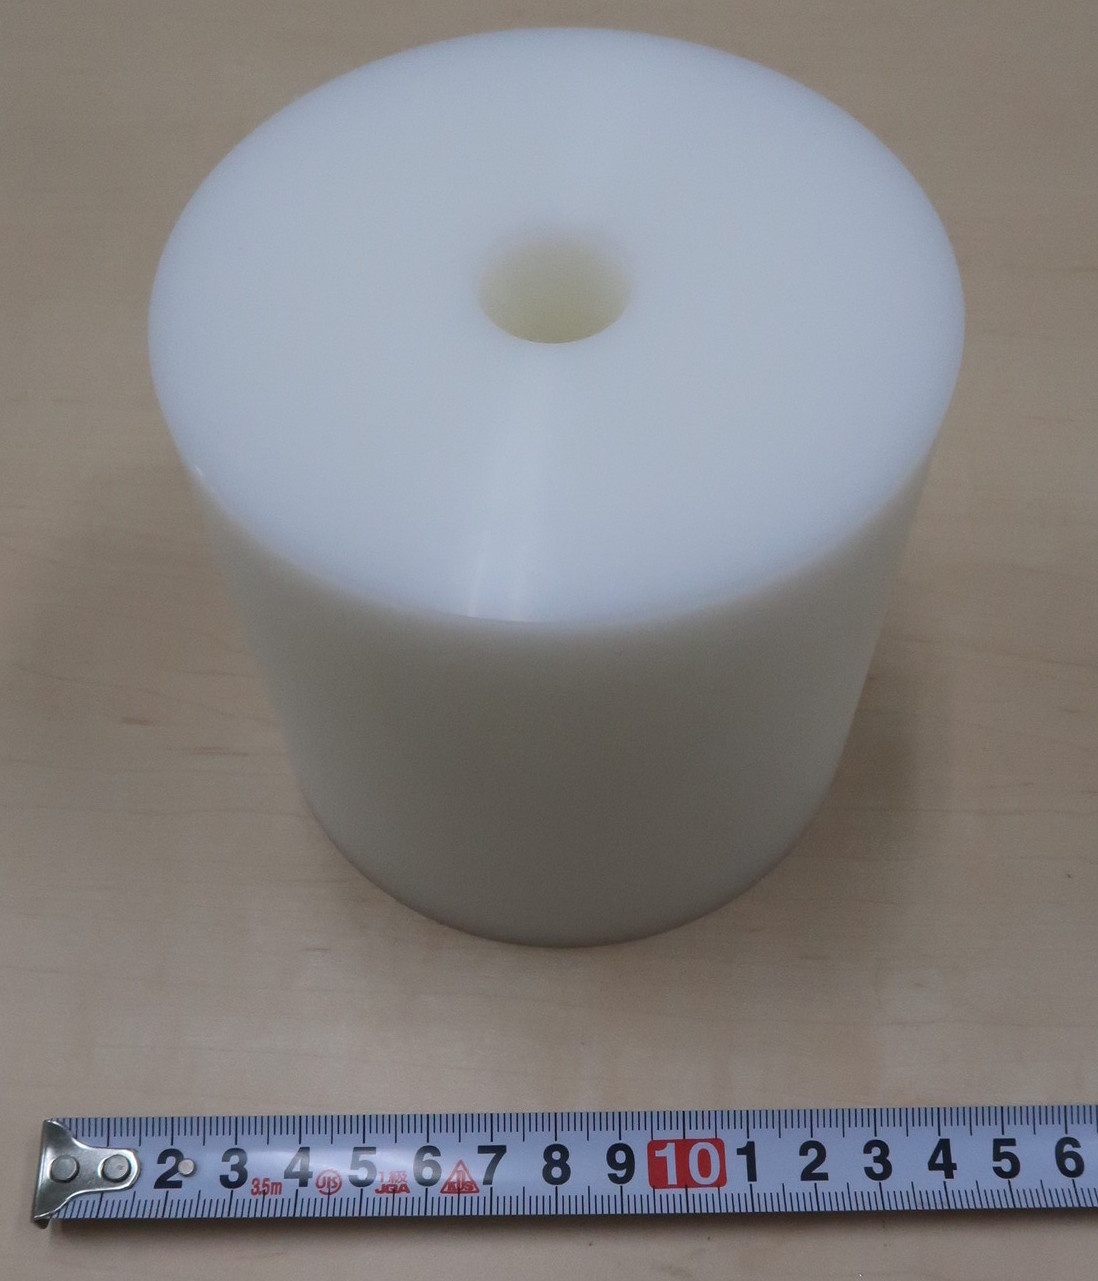
\includegraphics[clip, width=0.8\columnwidth]{IMG_2755_clpd.jpg}
  \caption[ポリエチレンで作成したコリメータ.]
          {ポリエチレンで作成したコリメータ.
            半径\SI{53}{\milli\metre},長さ\SI{100}{\milli\metre}の円柱の中央に,
          半径\SI{1}{\milli\metre}の穴が開いている.}
  \label{pic::collimator}
\end{figure}

\section{中性子の収量}
PHITS による計算では\SIrange{0}{10}{\milli\metre}の範囲の
\SIrange{13.9}{14.1}{\mega\electronvolt}の中性子は
\SI{4.07e-5}{\per\mega\electronvolt\per source}となる.
OKTAVIAN のDCビームラインで生成される中性子が\SI{5e9}{\per\second}であるとすると,
コリメータを通過してくる中性子の収量は\SI{4.07e4}{\per\second}となる.
\end{document}
